The \textcolor{darkblue}{Multitouch} library is able to suit different setups 
\& needs by loading modules which change its behavior.

The library architecture remains simple and provides two main entities:
\begin{itemize}
\item \textit{inputs} that generate packets.
\item \textit{outputs} that are responsible of final processing on packets. 
\end{itemize}
An application can enable as many inputs \& outputs as needed, may use
them independently or bind inputs to outputs (this is the standard
behavior as shown in the image).
\begin{center}
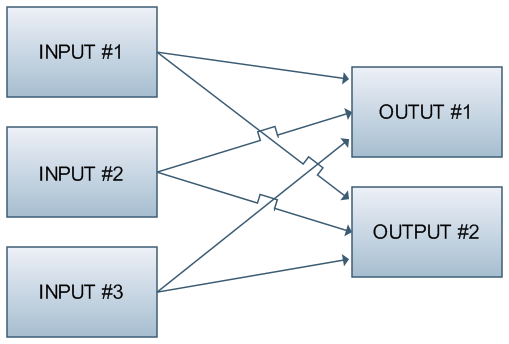
\includegraphics[keepaspectratio=true, width=200pt]{images/arch.png}
\end{center}

Also as you can see in the following image, inputs transmit 
packets to processing engines before making them available to the application
(or straight to outputs), and outputs pass the packets they receive from the 
application (or directly from inputs) to processing engines too, before doing 
own processing on them.
\begin{center}
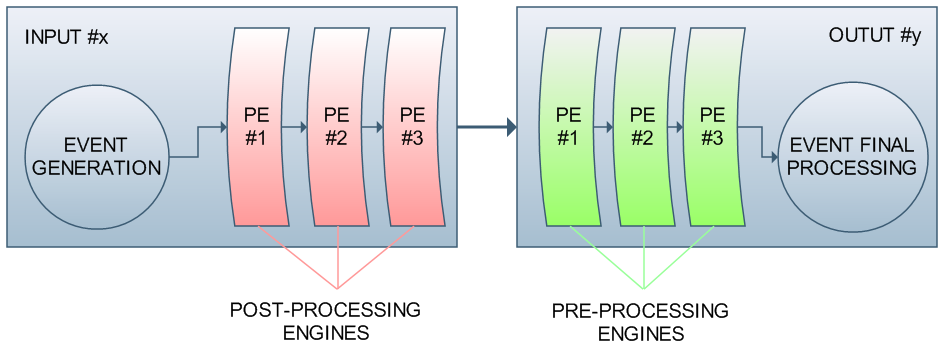
\includegraphics[keepaspectratio=true, width=\textwidth]{images/arch_pe.png}
\end{center}

To customize the inputs, outputs and processing engines to fit your
requirements and hardware, you have to write drivers (a driver is 
composed of three \texttt{C} functions which respect a defined prototype).

Thanks to this modular design and drivers, you could use the 
\textcolor{darkblue}{Multitouch} library to offer to an application 
the possibility to:
\begin{itemize}
\item Get datas from a touchpad or from more than one device (using or 
\textbf{not}, the same driver).
\item Write datas into a file.
\item Merge them and send it over the network
\item Emulate a kernel driver by creating a device on the file system feeded 
by data collected over the network
\item ect..
\end{itemize}

This guide cover all the aspects of the customization of the libary by a
developer, thus it:
\begin{enumerate}
\item Explains how to write a module.
\item Describes inputs drivers. 
\item Describes outputs drivers. 
\item Describes processing engine hook points. 
\end{enumerate}
